\documentclass{beamer}

\usetheme{Madrid}

\usepackage[english]{babel}

\usepackage{amsmath,amsthm,amssymb}
\usepackage{bbold}
\usepackage{graphicx}
\usepackage{listings}
\usepackage{multicol}
\usepackage{setspace}
\usepackage{xcolor}
%\usepackage{enumitem}
\usepackage{float}
% Common set symbols
\newcommand{\Z}{\mathbb{Z}}
\newcommand{\N}{\mathbb{N}}
\newcommand{\R}{\mathbb{R}}
\newcommand{\Q}{\mathbb{Q}}
\newcommand{\C}{\mathbb{C}}
\newcommand{\B}{\mathbb{B}}
\newcommand{\nullset}{\varnothing}
\newcommand{\powerset}[1]{\mathcal{P} ({#1})}
\newcommand{\ol}[1]{\overline{#1}}
\newcommand{\floor}[2]{\lfloor \frac{#1}{#2} \rfloor}

\newcommand{\email}{\href{mailto:MicahJSherry@gmail.com}{MicahJSherry@gmail.com}}
\newcommand{\name}{Micah Sherry}

\title[\email]{Factorization of Polynomials\\ Over the Boolean Semifield }
\subtitle{\small MAA Student Talk}

\author[\name]{
    \name \\
    \email
}
\setbeamertemplate{bibliography item}{\insertbiblabel}
\setbeamertemplate{navigation symbols}{}
%\setbeamertemplate{footline}{}

\setbeamertemplate{navigation symbols}{} % Optional: removes nav symbols



\date{March 27, 2026}
\begin{document}

    \begin{frame}
        \titlepage
    \end{frame}
    
    \begin{frame}{Background}
        The Boolean semifield, denoted as $\B$, is an algebraic structure with two operations: logical OR, analogous to addition, and
        logical AND, analogous to multiplication. $\B$ the only finite semifield that is not a field. Our research explores the factorization of polynomials over the Boolean semifield, denoted as $\B[x]$.  
        
        A key challenge in $\B[x]$ is that factorization is not unique. Specifically, we investigate the factorization of a particular
        class of polynomials in $\B[x]$ namely: $$f_n(x) = \sum_{i=0}^{n} x^i = x^n + x^{n-1} + \cdots + x + 1$$
        
        Understanding the non-unique factorization of these polynomials is a central focus of our study. This research contributes to a
        deeper understanding of algebraic structures beyond traditional fields and rings. 
    \end{frame}
    
    \begin{frame}{Definitions}
        \begin{itemize}
            \item A semifield is an algebraic structure like a field with addition and multiplication. 
                That does not necessarily have additive inverses and does have multiplicative inverses. 
            \item Let $\B = \{0, 1\}$ be the Boolean semifield equipped with logical OR as addition and Logical AND as Multiplication.  
            \item Let $\B[x]$ be the set of all polynomials in $x$ over $\B$.
            \item Let $f_n(x)\in \B[x]$, be defined as $f_n(x) = x^n +x^{n-1}+\cdots + x +1$.
        \end{itemize}
    \end{frame}

    %\begin{frame}{Related Topics}
    %    \begin{enumerate}
    %        \item Set Addition\\
    %            $A+B = \{a+b|a \in A \text{ and } b \in B\}$ where $A,B \subseteq \N$
    %        \item Dismal Arithmetic (base $b \ge 2$)
    %            Let $a$ and $b$ be base-$b$ numbers with digits in $\{0,1,\dots,b-1\}$.
    %            \begin{enumerate}
    %                \item $a \oplus b$ is given by digitwise $\max$ (no carries).
    %                \item $a \otimes b$ is given by digitwise $\min$, combined as in ordinary multiplication (no carries).
    %            \end{enumerate} 
    %        \item Numbral Arithmetic
    %            let $a$ and $b$ be binary sequences.
    %            \begin{enumerate}    
    %                \item $a+b$ is given by Bitwise OR.
    %                \item $a \times b$ is given by Shift-and-OR.
    %            \end{enumerate}
    %        \item Polynomials in $x$ over the Tropical semiring
    %    \end{enumerate}
    %\end{frame}


\begin{frame}{Necessary but Not Sufficient Condition for Factorization}
\small
\begin{theorem}
Let $\displaystyle f(x)=\sum_{i=0}^{n} f_i x^i$ with $f_0=1$.
    If $f(x)$ is factorable, then there exist $j,k$ with $\displaystyle 1 \le j,k\le n-1$ and $j+k=n$ such that $f_j=f_k=1$.
\end{theorem}

\begin{proof}
Assume $f(x)=g(x)h(x)$ with $1\le \deg(g),\deg(h)\le n-1 $. Let $\deg(g)=j$, $\deg(h)=k$. Then  
$\displaystyle g(x)=x^j+g'(x)+1,\quad h(x)=x^k+h'(x)+1$.
\begin{align*}
    f(x) &=g(x)h(x)\\
    &=(x^j+g'(x)+1)(x^k+h'(x)+1)\\
    &= x^{j+k}+x^j+x^k + \big(x^j h'(x)+x^k g'(x)+g'(x)h'(x)+g'(x)+h'(x)\big)+1.
\end{align*}
Thus $j+k=n$ and $f_j=f_k=1$
\end{proof}

\medskip

\textbf{Remark.}  
$\displaystyle f(x)=x^6+x^4+x^2+x+1$ satisfies the condition but is not factorable.

\end{frame}

   
\begin{frame}{Examples of Possible Factorization }    
        \begin{tabular}{|l||l|l|}
            \hline
            n & $f_n(x)$ & Factorizations \\
            \hline\hline
            2 & $x^2 + x + 1$ & $(x + 1)^2$ \\
            \hline
            3 & $x^3 + x^2 + x + 1$ & $(x + 1)^3$ \\
            & & $(x + 1)(x^2 + 1)$ \\
            \hline
            4 & $x^4 + x^3 + x^2 + x + 1$ & $(x + 1)^4$ \\
            & & $(x + 1)^2(x^2 + 1)$ \\
            & & $(x^3 + x + 1)(x + 1)$ \\
            & & $(x + 1)(x^3 + x^2 + 1)$ \\
            \hline
            5 & $x^5 + x^4 + x^3 + x^2 + x + 1$ & $(x + 1)^5$ \\
            & & $(x + 1)^3(x^2 + 1)$ \\
            & & $(x^3 + x + 1)(x + 1)^2$ \\
            & & $(x + 1)^2(x^3 + x^2 + 1)$ \\
            & & $(x + 1)(x^2 + 1)^2$ \\
            & & $(x + 1)(x^4 + x^2 + x + 1)$ \\
            & & $(x^3 + 1)(x + 1)^2$ \\
            & & $(x + 1)(x^4 + x^3 + x^2 + 1)$ \\
            \hline
        \end{tabular}
    \end{frame}
    
    \begin{frame}{Exponential Growth of Factors}
            \begin{figure}[h!]
                \centering
                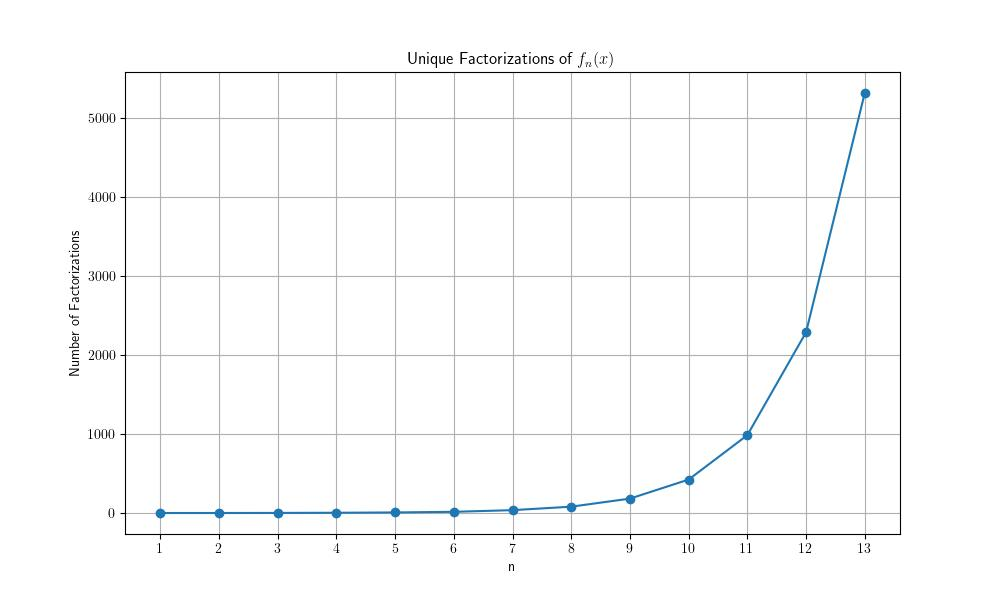
\includegraphics[width=1\textwidth]{factorization.jpg}
            \end{figure}
    \end{frame}
            
    \begin{frame}{Growth Rate of Factors}
            \begin{figure}[h!]
                \centering
                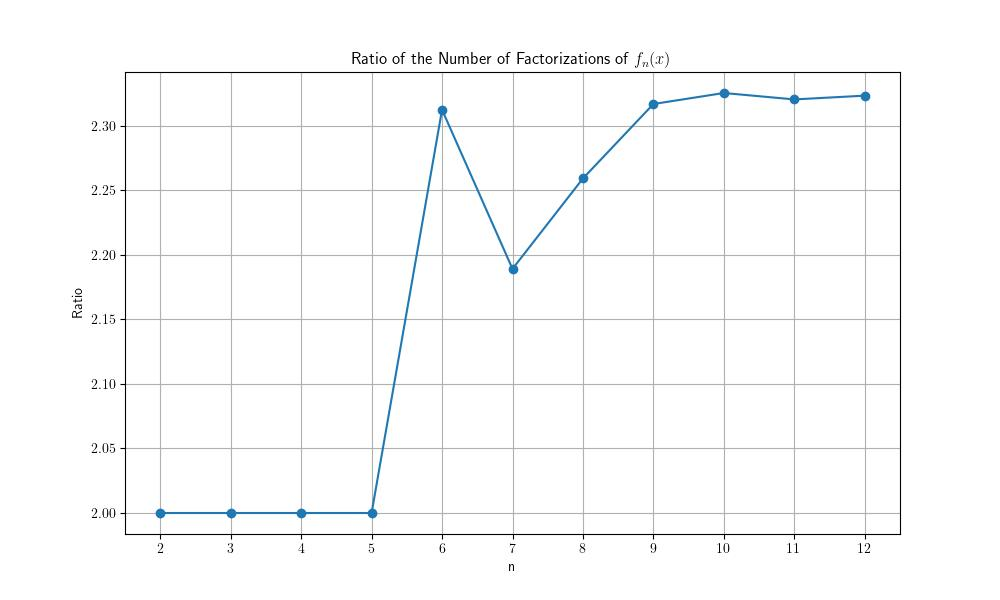
\includegraphics[width=1\textwidth]{ratio.jpg}
            \end{figure}
    \end{frame}
    



    \begin{frame}[shrink=6]{Divisibility of $f_n(x)$}
        \begin{lemma}
            Lemma 3.1 from the paper 'On the Sequence A079500 and Its Combinatorial Interpretations' \cite{frosini2006sequence} 
            states conditions for divisibility in the numbral arithmetic: For each $n, d > 0$,
            it holds that $[d]$ is a divisor of $[2^n - 1]$ if and only if it ends with the digit 1,
            and it does not contain any subsequence of 0s having length greater than $n-k$, with $k$
            being the length of $[d]$.
        \end{lemma}
        \begin{theorem}
            Let $g(x) \in \B[x]$ such that the constant term of $g(x)$ is 1. If $\deg(g(x)) = k$
            and $2k-1 \leq n$, then $g(x)$ divides $f_n(x)$.
        \end{theorem}
        \begin{proof}
            Let $\theta(h(x))$ be the isomorphism between $\B[x]$ and the numbral arithmetic $\theta(h(x))= [h(2)]$.
            Assume $2k-1 \leq n$ and let $d = \theta(g(x))$ (notice $[d]$ is length $k+1$). Let $m$ be
            the maximum length of zeros in $[d]$. Notice $m \leq k-1$. Notice $\theta(f_n(x)) = 2^{n+1}-1$.
            By the above lemma, $d$ divides $2^{n+1}-1$ because $k-1 \leq n+1-(k+1)$, which is
            equivalent to $2k-1 \leq n$. And by applying $\theta^{-1}$ we see $g(x)$ divides $f_n(x)$.
        \end{proof} 

    \end{frame}


    \begin{frame}[shrink=15]{Factorizations Of The Form $(x+1)h(x)= f_n(x) $}
        \small
        \begin{theorem}
            $(x+1)h(x) = f_n(x)$ if and only if $ \displaystyle h(x) = \sum_{i=0}^{n-1}h_ix^i$ With $h_{n-1} = h_0 =  1$ and $h_{i}+h_{i-1} = 1$ for $0<i<n-1$. 
        \end{theorem}
        \begin{proof}
            \small
            ($\rightarrow$): Assume that $(x+1)h(x) = f_n(x)$ and let $h(x) = \sum_{i=0}^{n-1} h_i x^i$.
            (Notice $h_{n-1} = h_0 = 1$ otherwise it would contradict the assumption). Now assume
            for the sake of contradiction that there exists $k < n-1$ such that $h_k = h_{k-1} = 0$.
            Consider the following:
            \[(x+1)h(x) = x \sum_{i=0}^{n-1} h_i x^i + \sum_{i=0}^{n-1} h_i x^i.\]
            Notice the $k$ term will have coefficient $h_k + h_{k-1} = 0$,
            contradicting the original assumption.

            ($\leftarrow$): Assume $h(x) = \sum_{i=0}^{n-1} a_i x^i$ with $h_{n-1} = h_0 = 1$ and for
            all $h_i$,  $h_i+h_{i-1} = 1$. Consider the following:
            \[(x+1)h(x) = \sum_{i=0}^{n-1} a_i x^{i+1} + \sum_{i=0}^{n-1} a_i x^i = a_{n-1}x^n + \sum_{i=1}^{n-1}(a_{i-1}+a_i)x^i + a_0 = f_n(x).\]
            Therefore, the theorem holds.
        \end{proof}    
    \end{frame}
    
    


    
    \begin{frame}[shrink=5]{Factorizations Of The Form $(x+1)h(x)= f_n(x) (Cont.)$}

        \begin{theorem}
            Let $H_n = \{h(x)|(x+1) h(x) = f_n(x) \}$
            Let $F_n$ be the $n^{th}$ Fibonacci number.
            $|H_n| = F_{n}$ for $n \geq 1$ 
        \end{theorem}
        \begin{proof}[Proof (by Strong induction)]    
            \noindent $H_1 = \{1\}, \quad |G_1| = 1 = F_1$
            \enspace \& \enspace
            $H_2 = \{x+1\}, \quad |H_2| = 1 = F_2$
            
            Therefore the base cases hold. Assume that $|H_j| = F_{j}$ for all $j \in \{1, 2, \ldots, k\}$ for some $k$. 
            Let $h(x) \in H_{k+1}$. Notice $\deg(h(x))=k$ and $h_k=1$ consider the possible values for $h_{k-1}$.
                \begin{enumerate}
                    \item Case 1. $h_{k-1} = 1$. In which case $h(x)=x^k + h'(x)$ Where $h'(x) \in H_k$.
                    \item Case 2. $h_{k-1} = 0$, So $h_{k-2} = 1$. In which case $h(x)=x^k + 0x^{k-1}+ h''(x)$ Where $h''(x) \in H_{k-1}$. 
                \end{enumerate}
                So, $|H_{k+1}| = |H_k| + |H_{k-1}| = F_{k} + F_{k-1} = F_{k+1}$.
                Therefore, by the Principle of Mathematical Induction $|H_n| = F_{n}$ for all $n\ge1$.
        \end{proof}
    \end{frame}

    \begin{frame}{Factorizations Of The Form $(x^k+1)g(x)= f_n(x)$}  
        \fontsize{8pt}{2pt}\selectfont
        \begin{theorem}
            Let $G_{nk} = \{g(x)|(x^k+1) g(x)=f_n(x)\}$,
            let $m=n-3k+1$,
            let $q = \floor{m}{k}$,
            and let $r= m\mod k$.
            $$|G_{nk}| = (F_{q+3})^r \times (F_{q+2})^{k-r}$$
        \end{theorem}
        \begin{proof}[Sketch] 
            Consider $\displaystyle g(x) = \sum_{i=0}^{n-k}g_ix^i \in G_{nk}$.\vspace{-1em}
            \begin{align*}
            (x^k+1) g(x)
                & =  \sum_{i=0}^{n-k}g_i x^{i+k} + \sum_{i=0}^{n-k}g_i x^i\\
                & =  \sum_{i=k}^{n}g_{i-k} x^{i} + \sum_{i=0}^{n-k}g_i x^i\\
                & = \sum_{i=n-k+1}^{n}g_i x^{i} + \sum_{i=k}^{n-k}(g_{k} + g_{i-k}) x^{i} + \sum_{i=0}^{k-1}g_i x^i
                =f_n(x)
            \end{align*}
            Notice this implies $g_i= 1$ for $i \le k-1$ or $i \ge n-2k+1$ and $g_i+g_{i-k} = 1$ for $k \le i \le n-2k$
            \renewcommand{\qedsymbol}{}
        \end{proof}
    \end{frame}
    
    \begin{frame}[shrink=5]{Factorizations Of The Form $(x^k+1)g(x)= f_n(x)$ (Cont.)}
        \begin{proof}[Sketch] 
            Construct a partition the coefficients $h_i$ where $k\le i \le n-2k$.
            Let $g_i \in P_j$ if $i \equiv j \mod k$.
            \begin{table}[h]
                \centering
                \begin{tabular}{|c|ll|}
                \hline 
                    $P_0$ & $g_k, \ g_{2k}, \  \cdots$  & $i \equiv 0 \mod k$ \\ \hline
                    $P_1$ & $g_{k+1}, \ g_{2k+1}, \cdots$  & $i \equiv 1 \mod k$ \\ \hline
                    \vdots & \vdots & \vdots \\ \hline
                    $P_0$ & $g_{2k-1}, \ g_{3k-1}, \cdots$  & $i \equiv k-1 \mod k$ \\ \hline
                \end{tabular}
            \end{table}
            Let $m = n-3k+1$, $q= \floor{m}{k}$, and $r = m \mod k$. The length of $r$ of these partitions is $q+1$ and $k-r$ have length $q$.
            It can be shown that the number of options (where $g_i+g_{i-k}=1$) for $P_j$ of length $q$ is $F_{q+2}$.
            So, The number of valid polynomials is $(F_{q+3})^r \times (F_{q+2})^{k-r}$
            \renewcommand{\qedsymbol}{$\square$}
        \end{proof}
    \end{frame}


    


    %\begin{frame}{Current Work}
    %    \begin{enumerate}
    %        \item Establishing $\prod_{i=1}^{n}F_i$ as a lower bound of number of unique factors.
    %        \item Determining the factors of the form $(x^k+1)h(x)=f_n(x).$
    %    \end{enumerate}
    %\end{frame}
    

    \begin{frame}[shrink=15]{Sources}
        \small
        \begin{multicols}{2}
            \bibliographystyle{plain}
            \bibliography{ref}
            \nocite{*}
        \end{multicols}        
    \end{frame}
    
    \begin{frame}{Related Topics}
        \begin{enumerate}
            \item Set Addition\\
                $A+B = \{a+b|a \in A \text{ and } b \in B\}$ where $A,B \subseteq \N$
            \item Dismal Arithmetic (base $b \ge 2$)
                Let $a$ and $b$ be base-$b$ numbers with digits in $\{0,1,\dots,b-1\}$.
                \begin{enumerate}
                    \item $a \oplus b$ is given by digitwise $\max$ (no carries).
                    \item $a \otimes b$ is given by digitwise $\min$, combined as in ordinary multiplication (no carries).
                \end{enumerate} 
            \item Numbral Arithmetic
                let $a$ and $b$ be binary sequences.
                \begin{enumerate}    
                    \item $a+b$ is given by Bitwise OR.
                    \item $a \times b$ is given by Shift-and-OR.
                \end{enumerate}
            \item Polynomials in $x$ over the Tropical semiring
        \end{enumerate}
    \end{frame}


\end{document}
